\chapter{Khởi động - xác định dự án (Task 1)}
\label{chap:task1}

\section{Tham vấn client và Client Interaction Log}
\label{sec:1-1}

Thầy Nguyễn Minh Tâm đóng vai client của dự án (P01). Các vòng trao đổi đến thời điểm hiện tại:

\begingroup\tblsetup\tblzebra
\begin{longtable}{L{1.6cm}L{3.2cm}L{3.2cm}L{6.0cm}}
\caption{Các vòng trao đổi với client}\label{tab:client-rounds}\\
\toprule
\rowcolor{tblheadbg}\textbf{Vòng} & \textbf{Gửi} & \textbf{Client trả lời} & \textbf{Nội dung} \\
\midrule
\endfirsthead
\toprule
\rowcolor{tblheadbg}\textbf{Vòng} & \textbf{Gửi} & \textbf{Client trả lời} & \textbf{Nội dung} \\
\midrule
\endhead
\bottomrule
\endlastfoot
P01 & 23/09/2026 20:25, Nguyễn Đức Nghĩa & 24/09/2026 07:48 & Vai trò client \\
Q01--Q09 & 02/10/2026 15:17, Nguyễn Đức Nghĩa & 02/10/2026 19:48 & Nghiệm thu, điểm danh, số chỗ/waitlist, tổ chức sự kiện, đăng nhập, báo cáo, quy mô, ràng buộc, hiện trạng \\
Q10--Q17, Q19--Q20 & 08/10/2026 16:39, Nguyễn Đức Nghĩa & 08/10/2026 19:58 & Xác nhận scope và MoE; role duyệt, hạn hủy, waitlist, đăng ký trùng, sửa/hủy sự kiện, quyền xem dữ liệu; milestone môn học; change event \\
Q21--Q22 (A58) & 23/10/2026 15:10, Nguyễn Đức Nghĩa & 25/10/2026 07:32 & Phạm vi demo tại Progress Check 09/11; kênh thông báo tối thiểu \\
\end{longtable}
\endgroup

Câu hỏi vòng 1 được chia theo 3 mức ưu tiên dựa trên tác động: mức 1 tác động lớn tới scope và rủi ro (Q08, Q03, Q04); mức 2 tác động tới luồng dữ liệu và thiết kế (Q01, Q02, Q05); mức 3 phục vụ giả định và đo lường (Q06, Q09, Q07). Mỗi câu hỏi mức 1--2 có kèm phân tích tác động và câu hỏi follow-up chuẩn bị trước. Nội dung đầy đủ của từng lần trao đổi ở Phụ lục~\ref{app:client-log}.

Vòng 2 (phản hồi ngày 08/10) xác nhận phạm vi và mục tiêu (Q10, Q11), chốt các quy tắc nghiệp vụ (Q12--Q15, Q19, Q20) và làm rõ lịch môn học (Q16, Q17). Các thay đổi chính đối với dự án:
\begin{itemize}
  \item Admin hệ thống thực hiện việc duyệt sự kiện, không tách thêm role riêng; Organizer không được tự duyệt sự kiện của mình (Q12).
  \item Hạn hủy đăng ký cố định 24 giờ trước giờ bắt đầu sự kiện (Q13).
  \item Organizer được sửa hoặc hủy sự kiện đã công bố; hệ thống phải thông báo người đã đăng ký khi đổi thời gian hoặc địa điểm (Q19). Đây là yêu cầu mới so với vòng 1.
  \item Môn học không có Milestone 2 và 3, chỉ có một lần Progress Check theo kế hoạch (Q16).
  \item Change event không báo trước nội dung; nhóm xem là rủi ro và dành contingency, không tạo trước activity riêng (Q17).
\end{itemize}

Vòng 2 gửi lúc 16:39 và được thầy trả lời lúc 19:58 cùng ngày 08/10; ảnh bằng chứng \texttt{Q10-Q20-2026-10-08-email-tra-loi.png} (P06) lưu trong thư mục minh chứng trên Drive của nhóm (Phụ lục~\ref{app:repository}).

\kiemtra{Cột \enquote{Tác động} ở Phụ lục~\ref{app:client-log} cho vòng 2 là đề xuất của AI, TV1 rà lại.}

Vòng 3 (A58) được gửi khi lịch A21 cho thấy đến 09/11 chưa có QR check-in; thầy trả lời sáng 25/10, trước họp A23. Thầy đồng ý phạm vi nhóm đề xuất (Q21): tại Progress Check chưa bắt buộc hoàn thiện toàn bộ workflow, gồm QR check-in và báo cáo/Excel/CSV, nhưng chức năng đã hoàn thành phải có bản demo chạy được, không chỉ trình bày giao diện hoặc mô tả thiết kế; chức năng đang phát triển phải thể hiện rõ tiến độ và kế hoạch hoàn thành. Thầy đồng ý thông báo trong ứng dụng là mức bắt buộc, email là mức Should (Q22). Nhóm sửa tiêu chí CP4 (mục~\ref{sec:2-5}) theo Q21, không đổi thứ tự công việc.

\kiemtra{Ảnh chụp email trả lời Q21, Q22 (TV1 cung cấp 27/10) cần lưu lên Drive làm bằng chứng (P06), đề xuất tên \texttt{Q21-Q22-2026-10-25-email-tra-loi.png}.}

\todo{Bổ sung: bằng chứng client đã làm thay đổi quyết định (scope, estimate, risk) cụ thể ra sao ở Baseline V1.0.}

\section{Bối cảnh, giả định và ràng buộc}
\label{sec:1-2}

\subsection*{Bối cảnh tổ chức}
Trường thường xuyên tổ chức seminar, workshop và hoạt động cho sinh viên. Sự kiện có thể do Khoa, CLB/Đội/Nhóm và các đơn vị/phòng ban của trường tổ chức. Các đơn vị này có thể tạo sự kiện, nhưng sự kiện phải được một vai trò có thẩm quyền (authorized role) phê duyệt trước khi công bố (Q01). Sinh viên là nhóm người tham gia chính; Organizer (Ban tổ chức) và Admin (quản trị viên hệ thống, đồng thời duyệt sự kiện) quản lý thông tin sự kiện và dữ liệu tham dự.

Quy trình hiện tại dùng form/bảng tính và có một số bước tổng hợp thủ công (Q07). Đây là planning assumption, không phải số liệu đo thực tế của nhà trường.

\subsection*{Vấn đề và cơ hội}
Thông tin sự kiện, đăng ký tham dự và điểm danh đang được quản lý bằng nhiều công cụ khác nhau. Workflow phân mảnh có thể buộc Ban tổ chức đối soát thủ công dữ liệu đăng ký, sức chứa, danh sách chờ (waitlist), điểm danh và báo cáo sau sự kiện. Cơ hội của dự án là xây dựng một hệ thống web responsive duy nhất, duy trì trạng thái người tham gia nhất quán từ khi sự kiện được công bố, qua đăng ký, điểm danh, đến báo cáo.

\subsection*{Sản phẩm đề xuất và hướng đã xác nhận}
\begin{itemize}
  \item Ứng dụng web responsive; không bắt buộc ứng dụng mobile native (Q09).
  \item Đăng nhập mô phỏng tài khoản trường bằng tài khoản mẫu có email trường (ASM-06); không tích hợp SSO thật (Q02).
  \item Phân quyền theo vai trò (RBAC) cho Student, Organizer và Admin; sự kiện phải được Admin duyệt trước khi công bố, Organizer không được tự duyệt sự kiện của mình (Q01, Q09, Q12). Organizer chỉ xem dữ liệu sự kiện do mình quản lý; Admin xem dữ liệu các đơn vị được giao duyệt; sinh viên chỉ xem đăng ký của chính mình (Q20).
  \item Quản lý số chỗ, đăng ký/hủy, waitlist; khi có chỗ trống tự động chuyển người đứng đầu waitlist sang danh sách đăng ký và thông báo cho người đó (Q04). Hủy được đến 24 giờ trước giờ bắt đầu (Q13); thông báo thất bại vẫn tính là đã đăng ký, không có trạng thái chờ xác nhận (Q14); sinh viên đã hủy được đăng ký lại, vào cuối waitlist nếu sự kiện đã đầy (Q15).
  \item Organizer được sửa hoặc hủy sự kiện đã công bố; đổi thời gian hoặc địa điểm thì thông báo người đã đăng ký; hủy sự kiện thì hủy các đăng ký, đóng waitlist và thông báo (Q19).
  \item Điểm danh bằng QR, có phương án dự phòng nhập mã hoặc xác nhận thủ công; không yêu cầu check-out (Q03).
  \item Báo cáo gồm danh sách đăng ký, danh sách điểm danh, thống kê số lượng tham gia, xuất Excel/CSV; tích hợp trực tiếp với hệ thống điểm rèn luyện nằm ngoài scope (Q05).
  \item Nhắc lịch/thông báo chung là chức năng bổ trợ; client ưu tiên core workflow hơn (Q08).
\end{itemize}

\subsection*{Giả định}
\begingroup\tblsetup\tblzebra
\begin{longtable}{L{1.5cm}L{6.5cm}L{1.5cm}L{3.5cm}}
\caption{Các giả định của dự án}\label{tab:assumptions}\\
\toprule
\rowcolor{tblheadbg}\textbf{Mã} & \textbf{Nội dung} & \textbf{Cơ sở} & \textbf{Trạng thái} \\
\midrule
\endfirsthead
\toprule
\rowcolor{tblheadbg}\textbf{Mã} & \textbf{Nội dung} & \textbf{Cơ sở} & \textbf{Trạng thái} \\
\midrule
\endhead
\bottomrule
\endlastfoot
ASM-01 & Quy trình hiện tại dùng form/bảng tính, có một số bước tổng hợp thủ công. & Q07 & Client cho phép giả định \\
ASM-02 & Không có số liệu sử dụng thực tế (Q06). Nhóm giả định để thiết kế và kiểm thử: khoảng 20 sự kiện mỗi tháng trên toàn hệ thống; trung bình 100 và tối đa 500 người đăng ký mỗi sự kiện; tối đa 50 lượt check-in đồng thời; tối đa 100 lượt đăng ký đồng thời khi mở đăng ký. & Q06 & Giả định của nhóm; client cho phép \\
ASM-03 & Hạn chót hủy đăng ký: mốc cố định 24 giờ trước giờ bắt đầu sự kiện, áp dụng toàn hệ thống; sau mốc này sinh viên liên hệ Organizer. & Q04, Q13 & Client đồng ý (08/10) \\
ASM-04 & Admin hệ thống thực hiện việc duyệt, không tách role riêng; Organizer không tự duyệt sự kiện của mình. Mô hình: Student / Organizer / Admin. & Q01, Q12 & Client đồng ý nguyên tắc (08/10) \\
ASM-05 & Nếu cần hosting, nhóm dùng gói miễn phí hoặc môi trường tương đương vì client không đặt ràng buộc hosting. & Q09 & Giả định của nhóm; client không ràng buộc \\
ASM-06 & Tài khoản trường được mô phỏng bằng tài khoản mẫu có email trường (dạng \texttt{mã@hcmut.edu.vn}) và mật khẩu cục bộ, đủ ba vai trò Student, Organizer, Admin; không kết nối hệ thống của trường. & Q02 & Giả định của nhóm; client cho phép \\
ASM-07 & Mốc hiện trạng để so sánh MoE: điểm danh thủ công khoảng 15 giây mỗi người; tổng hợp sau sự kiện khoảng 20 phút mỗi sự kiện (O2, O3). Đây là số do nhóm đặt, không phải số đo thực. & Q07 & Giả định của nhóm; client cho phép \\
\end{longtable}
\endgroup

\kiemtra{Giá trị của ASM-02, ASM-06, ASM-07 do PM chốt ngày 12/10 dựa trên đề xuất của AI (đã ghi AI Log) và được ghi là giả định của nhóm vì client cho phép (Q02, Q06, Q07). Nhóm rà lại tính hợp lý và độ khớp với bộ kiểm thử 500 lượt đăng ký ở O3; giả định phải được dùng nhất quán ở Product Description, test plan và risk register.}

\subsection*{Ràng buộc}
\begin{itemize}
  \item \textbf{Lịch:} Milestone~1 trình bày ngày 05/10/2026; CP1 ngày 04/10/2026. Task~2 hoàn thành sau M1 và trước khi chốt Baseline V1.0. Theo thầy (08/10, Q16) môn học không có Milestone~2 và 3; chỉ có một lần Progress Check theo kế hoạch (09/11) và demo, viva ngày 07/12.
  \item \textbf{Nhân lực:} nhóm 5 sinh viên; công việc quản lý dự án và hiện thực dùng chung nguồn lực giới hạn.
  \item \textbf{Dữ liệu và quyền riêng tư:} cần phân quyền cơ bản và bảo vệ thông tin cá nhân của sinh viên (Q09).
  \item \textbf{Nền tảng:} web responsive là đủ; không yêu cầu mobile native (Q09).
  \item \textbf{Hosting:} client không áp đặt; lựa chọn triển khai là quyết định kỹ thuật của nhóm (Q09).
  \item \textbf{Bằng chứng:} Client Interaction Log phải lưu trao đổi và mốc thời gian thực tế; không cần biên bản có chữ ký riêng (P06).
\end{itemize}
\begin{itemize}
  \item \textbf{Công cụ:} GitHub, Jira và Google Sheet (mục~\ref{sec:1-7}); CI/CD do repo code đảm nhiệm.
  \item \textbf{Ngân sách:} không có ngân sách bằng tiền; vận hành dùng gói miễn phí (ASM-05).
\end{itemize}
Stack kỹ thuật được nhóm chốt tại họp ngày 18/10: React cho giao diện, Go cho API, PostgreSQL cho cơ sở dữ liệu. Trong nhóm đã có thành viên từng học và làm dự án với Go.

\kiemtra{Bổ sung kỹ năng của từng thành viên với React, Go, PostgreSQL (chưa dùng, đã học, đã làm dự án) nếu cần cho phân công và rủi ro.}

\section{Business case và quyết định go/no-go}
\label{sec:1-3}
\subsection*{Lợi ích kỳ vọng}
Hệ thống thay thế quy trình form/bảng tính và tổng hợp thủ công hiện tại (Q07, client cho phép giả định), giảm sai sót đối soát và tăng tốc điểm danh bằng QR. Mức cải thiện được đo bằng các MoE O1--O4 ở Bảng~\ref{tab:objectives}; mốc hiện trạng là planning assumption (mục~\ref{sec:1-2}).

\subsection*{Chi phí và bất lợi}
\begin{itemize}
  \item Công sức của 5 sinh viên trong thời gian môn học; effort chính thức được xác định ở Task~2 (A18), trước khi chốt Baseline V1.0; chi phí nhân công tính bằng giờ người, không quy đổi sang VND.
  \item Chi phí vận hành bằng tiền: 0 VND theo giả định dùng free-tier hosting (ASM-05, Q09).
  \item Các đơn vị (Khoa, CLB/Đội/Nhóm) cần thời gian làm quen hệ thống; xử lý bằng tài liệu hướng dẫn giao diện. Nhóm đánh giá mức rủi ro thấp.
  \item Phạm vi giới hạn: không SSO thật, không tích hợp hệ thống điểm rèn luyện.
\end{itemize}

\subsection*{Phương án thay thế}
Giữ form/bảng tính như hiện trạng (Q07): không tốn công xây dựng nhưng vẫn phải đối soát thủ công. Việc dùng công cụ có sẵn chưa được nhóm khảo sát.

\subsection*{Tiêu chí và kết luận go/no-go}
Chưa áp dụng đánh giá tài chính (NPV, ROI) vì không có số liệu thực tế. Khuyến nghị: \textbf{GO}, vì chi phí vận hành bằng tiền bằng 0 (theo giả định free-tier) và hệ thống giải quyết đúng điểm đau thủ công hiện tại. Quyết định được đánh giá lại khi chốt Baseline V1.0, vì ước lượng effort chính thức chỉ có ở Task~2.

\textbf{Go nếu:}
\begin{itemize}
  \item Workflow cốt lõi rõ và được client xác nhận (Q08).
  \item Chi phí vận hành bằng tiền bằng 0 theo giả định free-tier (ASM-05).
  \item Không phụ thuộc hệ thống ngoài: không SSO thật, không tích hợp điểm rèn luyện (Q02, Q05).
\end{itemize}

\textbf{No-go nếu} (xét lại ở Baseline V1.0):
\begin{itemize}
  \item Client đổi hướng ưu tiên lớn hoặc yêu cầu tích hợp hệ thống ngoài.
  \item Effort ước lượng ở Task~2 vượt khả năng của 5 sinh viên, hoặc lịch vượt Progress Check 09/11 mà không thu hồi được.
\end{itemize}
\textbf{Xử lý khi no-go:} họp với client để thu hẹp scope, bỏ nhóm Could rồi Should (Bảng~\ref{tab:moscow}) trước, không bỏ core workflow.

Kết luận GO và các tiêu chí go/no-go ở trên đã được TV4 (phụ trách A06) xác nhận trong báo cáo Milestone~1.


Hướng xử lý (PM chốt 13/10): nếu ước lượng hoặc lịch của Task~2 vượt khả năng của 5 sinh viên hoặc vượt Progress Check 09/11 thì thu hẹp phạm vi theo thứ tự Could rồi Should, không bỏ core workflow. Bản đề xuất sơ bộ (nháp AI) cho thấy lịch có thể vượt, nên kết luận GO hiện là khuyến nghị có điều kiện.

\section{Phạm vi, loại trừ, mục tiêu và thước đo hiệu quả (MoE)}
\label{sec:1-4}

\subsection*{Phạm vi}
Dự án cung cấp hệ thống đăng ký và quản lý sự kiện dạng web responsive, bao phủ các workflow cốt lõi mà client ưu tiên nghiệm thu theo thứ tự (Q08):
\begin{enumerate}
  \item Tạo và quản lý sự kiện; sự kiện phải được Admin duyệt trước khi công bố, Organizer không được tự duyệt sự kiện của mình (Q01, Q12).
  \item Sinh viên đăng ký và hủy đăng ký; hủy được đến 24 giờ trước giờ bắt đầu (Q13); mỗi sinh viên chỉ có một đăng ký còn hiệu lực cho một sự kiện, hủy rồi được đăng ký lại (Q15).
  \item Quản lý số lượng và danh sách chờ: sự kiện có giới hạn số chỗ; khi có chỗ trống, hệ thống tự động chuyển người đầu waitlist sang danh sách đăng ký và gửi thông báo, không cần ban tổ chức duyệt lại (Q04); thông báo thất bại vẫn tính là đã đăng ký (Q14).
  \item Điểm danh bằng QR, có phương án dự phòng nhập mã hoặc xác nhận thủ công (Q03).
  \item Xem kết quả và báo cáo: danh sách đăng ký, danh sách điểm danh, thống kê số người tham gia; có thể xuất Excel/CSV (Q05).
\end{enumerate}
Thông báo và nhắc lịch là chức năng bổ trợ, ưu tiên thấp hơn các workflow trên (Q08). Ngoài ra, theo phản hồi 08/10 (Q19), Organizer được sửa hoặc hủy sự kiện đã công bố; khi đó hệ thống thông báo người đã đăng ký (đổi thời gian hoặc địa điểm) hoặc hủy đăng ký và đóng waitlist (hủy sự kiện).

\subsection*{Phân loại MoSCoW}
\begingroup\tblsetup\tblzebra
\begin{longtable}{L{1.8cm}L{10.2cm}L{1.8cm}}
\caption{Phân loại yêu cầu theo MoSCoW}\label{tab:moscow}\\
\toprule
\rowcolor{tblheadbg}\textbf{Mã} & \textbf{Yêu cầu} & \textbf{Mức} \\
\midrule
\endfirsthead
\toprule
\rowcolor{tblheadbg}\textbf{Mã} & \textbf{Yêu cầu} & \textbf{Mức} \\
\midrule
\endhead
\bottomrule
\endlastfoot
REQ-01 & Đăng nhập mô phỏng tài khoản trường & Must \\
REQ-02 & Truy cập và xem dữ liệu theo vai trò cho Student / Organizer / Admin (Q12, Q20) & Must \\
REQ-03 & Tạo/chỉnh sửa sự kiện & Must \\
REQ-04 & Phê duyệt trước khi công bố (Admin duyệt; Organizer không tự duyệt) & Must \\
REQ-05 & Giới hạn số lượng đăng ký (capacity) & Must \\
REQ-06 & Đăng ký/hủy đăng ký & Must \\
REQ-07 & Danh sách chờ (waitlist) & Must \\
REQ-08 & Tự động chuyển người đầu waitlist khi có chỗ trống & Must \\
REQ-09 & Thông báo cho người được chuyển từ waitlist & Must \\
REQ-10 & Điểm danh bằng QR & Must \\
REQ-11 & Phương án dự phòng cho QR: nhập mã/xác nhận thủ công & Must \\
REQ-12 & Danh sách đăng ký và danh sách tham dự & Must \\
REQ-13 & Thống kê tham dự & Must \\
REQ-14 & Xuất Excel/CSV & Must \\
REQ-15 & Bảo vệ dữ liệu cá nhân cơ bản & Must \\
REQ-16 & Xác nhận đăng ký & Should \\
REQ-17 & Nhắc lịch/thông báo sự kiện (ngoài thông báo khi chuyển từ waitlist) & Should \\
REQ-18 & Thống kê sau sự kiện phong phú hơn & Should \\
REQ-19 & Phản hồi của người tham dự sau sự kiện & Could \\
REQ-20 & Cải tiến UI tiện dụng không ảnh hưởng core workflow & Could \\
REQ-21 & Sửa hoặc hủy sự kiện đã công bố; thông báo người đã đăng ký khi đổi thời gian hoặc địa điểm; hủy sự kiện thì hủy đăng ký và đóng waitlist (Q19) & Should \\
\end{longtable}
\endgroup

REQ-21 đặt mức Should (PM chốt 13/10). Thông báo khi chuyển từ waitlist (REQ-09) và khi sự kiện đổi hoặc hủy là bắt buộc; kênh tối thiểu là thông báo trong ứng dụng, gửi email là tùy chọn (nhóm đề xuất, thầy đồng ý ngày 25/10, Q22).

\subsection*{Loại trừ (Won't)}
\begin{itemize}
  \item Tích hợp SSO thật của trường/HCMUT (Q02).
  \item Ứng dụng native Android/iOS (Q09).
  \item Tích hợp trực tiếp với hệ thống điểm rèn luyện (Q05).
  \item Check-out bắt buộc (Q03).
  \item Đồng bộ offline đầy đủ.
  \item Cam kết khả năng mở rộng không giới hạn trong môi trường thực; các giá trị tải chỉ là giả định kiểm thử vì client không có số liệu quy mô thực tế (Q06).
\end{itemize}

\subsection*{Mục tiêu và MoE}
Các mốc hiện trạng dưới đây là planning assumption của nhóm, không phải số đo thực tế (xem Bảng~\ref{tab:assumptions}).

\begingroup\tblsetup\tblzebra
\begin{longtable}{L{0.9cm}L{3.8cm}L{4.0cm}L{5.3cm}}
\caption{Mục tiêu và thước đo hiệu quả}\label{tab:objectives}\\
\toprule
\rowcolor{tblheadbg}\textbf{Mã} & \textbf{Mục tiêu} & \textbf{Mốc hiện trạng (giả định)} & \textbf{Chỉ tiêu MoE} \\
\midrule
\endfirsthead
\toprule
\rowcolor{tblheadbg}\textbf{Mã} & \textbf{Mục tiêu} & \textbf{Mốc hiện trạng (giả định)} & \textbf{Chỉ tiêu MoE} \\
\midrule
\endhead
\bottomrule
\endlastfoot
O1 & Duy trì chính xác trạng thái đăng ký, số chỗ và waitlist với ít đối soát thủ công hơn & Workflow hiện tại có thể dùng form/bảng tính và tổng hợp thủ công (Q07); chưa có số đo tỷ lệ lỗi & 100\% acceptance test đạt; ngăn đăng ký trùng và vượt số chỗ; tự động chuyển waitlist đúng FIFO trong mọi test case đã định nghĩa \\
O2 & Tăng tốc điểm danh và vẫn hoạt động được khi QR/thiết bị/mạng gặp vấn đề & Chưa có số đo thực tế; giả định để so sánh: tra cứu/điểm danh thủ công $\approx$ 15 giây/người & Median điểm danh $\leq$ 5 giây trong môi trường test của nhóm; chặn điểm danh trùng; manual fallback cập nhật attendance giống QR \\
O3 & Giảm thời gian lấy thông tin tham dự sau sự kiện & Chưa có số đo thực tế; giả định tổng hợp thủ công $\approx$ 20 phút/sự kiện & Với bộ dữ liệu kiểm thử 500 lượt đăng ký, tổng hợp tham dự và xuất Excel/CSV xong trong 30 giây; số liệu khớp hoàn toàn dữ liệu nguồn \\
O4 & Chỉ vai trò có thẩm quyền mới publish được sự kiện hoặc truy cập chức năng hạn chế & Quy trình hiện tại chưa được đo & 100\% authorization test đạt; không sự kiện nào publish khi chưa qua vai trò duyệt; không còn lỗi nghiêm trọng về quyền riêng tư/kiểm soát truy cập tại UAT \\
\end{longtable}
\endgroup

\subsection*{Truy vết tới Client Log}
Q01 quyết định luồng duyệt sự kiện; Q02 giới hạn scope xác thực; Q03 xác định QR cùng phương án dự phòng và loại check-out; Q04 đưa số chỗ/waitlist/tự động chuyển vào core scope; Q05 xác định báo cáo/xuất dữ liệu và loại tích hợp điểm rèn luyện; Q06--Q07 cho phép dùng planning assumption được ghi rõ; Q08 xác định ưu tiên nghiệm thu của core workflow; Q09 xác nhận web responsive, phân quyền và bảo vệ dữ liệu cơ bản, không ràng buộc hosting. Vòng 2 (08/10): Q10--Q11 xác nhận scope, objective và MoE; Q12 chốt Admin duyệt; Q13 chốt hạn hủy 24 giờ; Q14--Q15 chốt quy tắc waitlist và đăng ký lại; Q19 thêm yêu cầu sửa/hủy sự kiện đã công bố; Q20 chốt quyền xem dữ liệu; Q16--Q17 làm rõ mốc môn học và change event.

\section{Thẩm quyền dự án}
\label{sec:1-5}
\subsection*{Các vai trò có thẩm quyền}
\begin{itemize}
  \item \textbf{Client/sponsor:} thầy Nguyễn Minh Tâm. Các vấn đề về scope, mức ưu tiên và thay đổi yêu cầu trao đổi trực tiếp với thầy (P01).
  \item \textbf{Project Manager:} Nguyễn Đức Nghĩa (TV1), chịu trách nhiệm liên hệ client, duyệt baseline, phân bổ tài nguyên, xử lý change request.
\end{itemize}

\subsection*{Trách nhiệm ra quyết định}

\begingroup\tblsetup\tblzebra
\begin{longtable}{L{6.0cm}L{4.0cm}L{4.0cm}}
\caption{Trách nhiệm ra quyết định}\label{tab:decision-rights}\\
\toprule
\rowcolor{tblheadbg}\textbf{Quyết định} & \textbf{Người quyết định} & \textbf{Người tham gia} \\
\midrule
\endfirsthead
\toprule
\rowcolor{tblheadbg}\textbf{Quyết định} & \textbf{Người quyết định} & \textbf{Người tham gia} \\
\midrule
\endhead
\bottomrule
\endlastfoot
Scope, mức ưu tiên, thay đổi yêu cầu & Client & PM (đề xuất) \\
Duyệt baseline & PM & Cả nhóm thống nhất trước khi duyệt \\
Giải pháp kỹ thuật trong phạm vi scope đã chốt & TV3 (Tech Lead) & TV4, TV5 \\
Phân bổ tài nguyên, change request & PM & Thành viên liên quan \\
Duyệt checkpoint & Theo Bảng~\ref{tab:checkpoints} & \\
\end{longtable}
\endgroup

\subsection*{Cơ chế leo thang}
Vấn đề được xử lý ở cấp thấp nhất có thể, theo thứ tự: thành viên phụ trách $\rightarrow$ PM $\rightarrow$ họp nhóm $\rightarrow$ client. Vấn đề được đưa lên họp nhóm khi gặp một trong các ngưỡng:
\begin{enumerate}
  \item Quyết định cần từ 3 người trở lên mà trao đổi trên chat chưa thống nhất.
  \item Độ lệch $>20\%$ ở activity nằm trên đường găng.
  \item Rủi ro có exposure $\geq 12$ xảy ra.
  \item Từ 2 người trở lên báo blocker trong cùng một đợt.
  \item Có change event.
  \item Trước checkpoint.
\end{enumerate}
Vấn đề ảnh hưởng đến scope, mức ưu tiên hoặc yêu cầu được PM chuyển lên client (P01).

\section{Phân tích các bên liên quan}
\label{sec:1-6}
Các bên liên quan rút ra từ đề tài và Client Log được phân tích ở Bảng~\ref{tab:stakeholder}. Mức ảnh hưởng và quan tâm là đề xuất của nhóm; nhóm không khảo sát sinh viên thật (P03) và chưa khẳng định đã tham vấn đại diện đơn vị tổ chức.

\begingroup\tblsetup\tblzebra
\begin{longtable}{L{2.4cm}L{3.2cm}L{1.9cm}L{1.3cm}L{5.2cm}}
\caption{Phân tích các bên liên quan}\label{tab:stakeholder}\\
\toprule
\rowcolor{tblheadbg}\textbf{Bên liên quan} & \textbf{Vai trò / quan tâm} & \textbf{Ảnh hưởng} & \textbf{Quan tâm} & \textbf{Chiến lược và kênh trao đổi} \\
\midrule
\endfirsthead
\toprule
\rowcolor{tblheadbg}\textbf{Bên liên quan} & \textbf{Vai trò / quan tâm} & \textbf{Ảnh hưởng} & \textbf{Quan tâm} & \textbf{Chiến lược và kênh trao đổi} \\
\midrule
\endhead
\bottomrule
\endlastfoot
Giảng viên Nguyễn Minh Tâm (client) & Quyết định scope, ưu tiên, thay đổi yêu cầu (P01); đã xác nhận workflow ưu tiên, duyệt trước khi công bố, waitlist tự động, QR có dự phòng & Cao & Cao & Trao đổi sát qua TV1 bằng email; ghi câu trả lời và tác động vào Client Log; đồng bộ scope và tiêu chí nghiệm thu \\
Đơn vị tổ chức sự kiện và người duyệt sự kiện & Tạo sự kiện, kiểm soát công bố, số chỗ và điểm danh (Q01); Admin hệ thống duyệt sự kiện, Organizer không tự duyệt sự kiện của mình (Q12) & Trung bình đến cao & Cao & Làm rõ quyền duyệt, công bố, quản lý chỗ và điểm danh trong thiết kế; bảo đảm chỉ sự kiện đã duyệt mới công bố và nhận đăng ký \\
Sinh viên tham dự & Đăng ký, hủy, vào waitlist và được điểm danh; chịu tác động trực tiếp & Thấp (với quyết định dự án) & Cao & Thiết kế và thử luồng bằng tài khoản, dữ liệu mô phỏng \\
Nhóm dự án (TV1--TV5) & Lập kế hoạch, triển khai, bảo vệ dữ liệu sinh viên, báo cáo tiến độ & Cao (với cách thực hiện) & Cao & Cùng chốt các quy tắc còn mở, review chéo, lưu bằng chứng theo mã activity; trao đổi qua chat, board và Sheet \\
\end{longtable}
\endgroup

\todo{Nêu thay đổi cụ thể về objective/scope/cách tiếp cận do phân tích stakeholder (nếu có); bổ sung bên liên quan khác nếu nhóm xác định thêm.}

\section{Hạ tầng dự án: tiêu chuẩn, tổ chức nhóm và giao tiếp}
\label{sec:1-7}

\subsection*{Tổ chức nhóm}

Nhóm phân vai lại tại họp ngày 18/10: TV1 phụ trách toàn bộ sản phẩm quản trị và báo cáo; TV2 kiểm thử; TV3 và TV5 backend; TV4 frontend. Các sản phẩm quản trị làm trước 18/10 vẫn ghi đúng người đã thực hiện theo phân công cũ.

\begingroup\tblsetup\tblzebra
\begin{longtable}{L{1.2cm}L{4.0cm}L{8.8cm}}
\caption{Vai trò và trách nhiệm}\label{tab:roles}\\
\toprule
\rowcolor{tblheadbg}\textbf{Mã} & \textbf{Vai trò} & \textbf{Sở hữu} \\
\midrule
\endfirsthead
\toprule
\rowcolor{tblheadbg}\textbf{Mã} & \textbf{Vai trò} & \textbf{Sở hữu} \\
\midrule
\endhead
\bottomrule
\endlastfoot
TV1 & Project Manager (Nguyễn Đức Nghĩa) & Toàn bộ sản phẩm quản trị và báo cáo: thẩm quyền dự án, Client Log, scope và MoE, business case, stakeholder, PBS/PFD, Product Descriptions, ước lượng, lịch và Gantt, tài nguyên, sổ rủi ro, quality plan, baseline, weekly log, truy vết, change request, AI log, báo cáo \\
TV2 & Tester (Ngô Thanh Hùng) & Test case, chạy kiểm thử, regression, hỗ trợ UAT \\
TV3 & Tech Lead, Backend (Phan Huy Quang Minh) & Quyết định kỹ thuật, cơ sở dữ liệu (PostgreSQL), API (Go) \\
TV4 & Frontend (Nguyễn Đắc Nghĩa) & Giao diện (React) \\
TV5 & Backend, DevOps (Hà Cao Đức Minh) & Backend (Go) cùng TV3, codebase, CI/CD, triển khai, điểm danh QR \\
\end{longtable}
\endgroup

\subsection*{Công cụ và hạ tầng}
\begingroup\tblsetup\tblzebra
\begin{longtable}{L{2.6cm}L{11.4cm}}
\caption{Công cụ quản lý dự án}\label{tab:tools}\\
\toprule
\rowcolor{tblheadbg}\textbf{Công cụ} & \textbf{Vai trò} \\
\midrule
\endfirsthead
\toprule
\rowcolor{tblheadbg}\textbf{Công cụ} & \textbf{Vai trò} \\
\midrule
\endhead
\bottomrule
\endlastfoot
GitHub (tổ chức \texttt{qldapm-hcmut}) & Kho mã nguồn (\texttt{ticket-system-uni}) và tài liệu quản lý (\texttt{pm-docs}); mỗi công việc làm trên nhánh riêng, đưa vào \texttt{main} qua Pull Request có người review \\
CI/CD của repo code & Build và test chạy trong repo \texttt{ticket-system-uni}, do người dựng repo thiết lập; nhóm không dựng CI riêng cho repo tài liệu \\
Jira & Space Uni-Ticket-System (key SCRUM), theo dõi công việc bằng sprint hằng tuần với trạng thái Backlog, In Progress, Done; thẻ gắn mã activity; worklog làm dữ liệu actual effort \\
Google Sheet Master & Client Log, Traceability, Estimates, Risk Register, Weekly Log, Time Tracking \\
Chat và thư mục tài liệu & Báo tiến độ, vướng mắc; thư mục phân quyền cho nhóm \\
\end{longtable}
\endgroup
Ban đầu nhóm dùng GitLab tự host (Merge Request) và Jenkins. Ngày 22/10 phát sinh I03 (mục~\ref{sec:3-4}): GitLab chạy trên máy cá nhân nên các thành viên khác chưa truy cập được. Sau đó nhóm chuyển sang GitHub (tổ chức \texttt{qldapm-hcmut}), đưa vào \texttt{main} qua Pull Request có người review; nguyên tắc review và lưu bằng chứng giữ nguyên. CI/CD do người dựng repo code thiết lập nên nhóm không dựng Jenkins hay CI riêng cho repo tài liệu; quyết định ``CI dùng Jenkins'' (21/10) không còn áp dụng.

\kiemtra{Ngày nhóm chuyển sang GitHub và ngày đóng I03 cần TV1 điền; mục 1.7 này mô tả hạ tầng tại thời điểm viết, cập nhật nếu CI/CD của repo code đổi.}

\kiemtra{Trước khi mirror: rà repo không chứa mật khẩu, khóa truy cập hoặc dữ liệu thật của sinh viên (tiêu chuẩn bảo mật ở mục này); tạo mirror và ghi link vào Phụ lục~\ref{app:repository}.}

\todo{Bổ sung ảnh chụp bằng chứng hạ tầng (cả 5 thành viên truy cập được, \texttt{main} được bảo vệ, một Pull Request mẫu có review); link board, Sheet và thư mục tài liệu ở Phụ lục~\ref{app:repository}.}

\subsection*{Kiến trúc kỹ thuật}
Stack được nhóm chốt tại CP2 ngày 18/10: frontend React (web responsive, không làm ứng dụng di động riêng theo Q09, Q10), backend Go, cơ sở dữ liệu PostgreSQL. Hình~\ref{fig:architecture} ánh xạ từng khối tới activity tạo ra nó; thiết kế bảng và hợp đồng API là sản phẩm của A25 (PD-02). CI/CD do repo code đảm nhiệm (thay quyết định dùng Jenkins ngày 21/10). Các phần chưa quyết định (nền tảng hosting, kênh thông báo ngoài ứng dụng) vẽ nét đứt.

\begin{figure}[H]
\centering
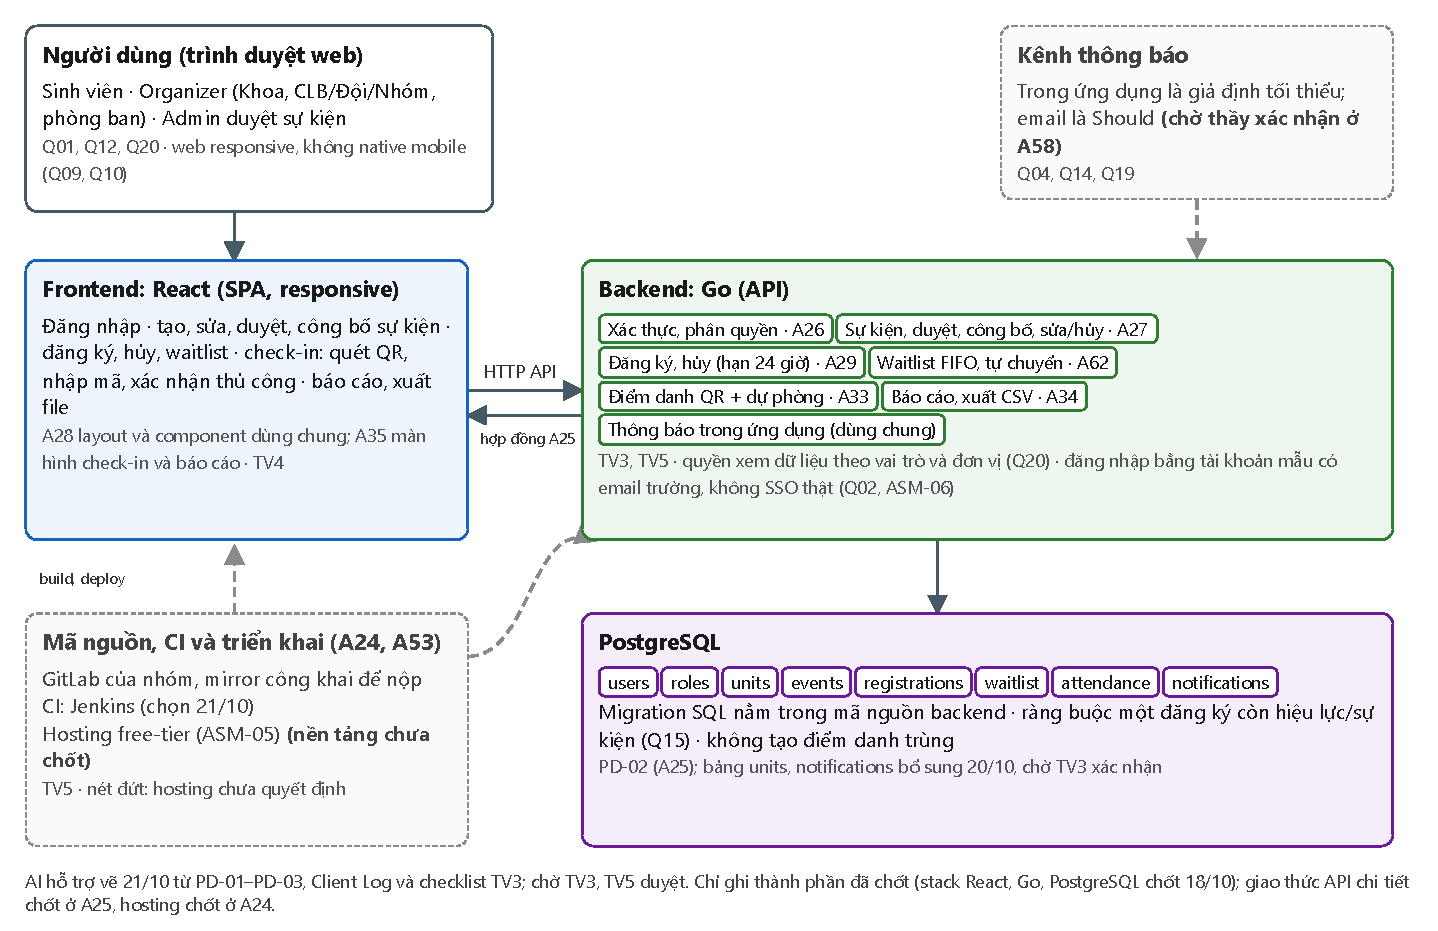
\includegraphics[width=\linewidth]{image/architecture.pdf}
\caption{Kiến trúc kỹ thuật React -- Go -- PostgreSQL và activity tương ứng}
\label{fig:architecture}
\end{figure}

\kiemtra{Hình~\ref{fig:architecture} do AI hỗ trợ vẽ ngày 21/10 từ PD-01 đến PD-03, Client Log và checklist TV3; chờ TV3, TV5 duyệt (nhất là phân chia module backend và bảng PostgreSQL).}

\subsection*{Kế hoạch giao tiếp}
\begin{itemize}
  \item \textbf{Với client:} qua email; TV1 là đầu mối, gom câu hỏi trước khi gửi; client không cam kết thời gian phản hồi (P02, P05). Mọi trao đổi ghi vào Client Log kèm mốc thời gian.
  \item \textbf{Trong nhóm:} dùng chat để báo tiến độ và vướng mắc bất đồng bộ; check-in 3 dòng vào thứ Tư/thứ Năm. TV1 tổng hợp tiến độ hằng tuần.
  \item \textbf{Công cụ theo dõi:} board Jira theo dõi công việc theo mã activity; Sheet Master ghi thời gian và bằng chứng.
  \item \textbf{Họp định kỳ:} 15h00 Chủ nhật hằng tuần, để rà soát time tracking, chốt weekly log, review chéo tài liệu và chuẩn bị cho viva.
  \item \textbf{Họp bất thường:} thêm khi gặp một trong các ngưỡng ở mục~\ref{sec:1-5}.
\end{itemize}

\subsection*{Tiêu chuẩn và quy trình}
\begin{itemize}
  \item \textbf{Git:} mỗi công việc một nhánh; Pull Request ghi mã công việc, nội dung thay đổi, cách kiểm tra; ít nhất một thành viên khác review trước khi vào \texttt{main}.
  \item \textbf{Bảo mật:} không đưa mật khẩu, khóa truy cập hoặc dữ liệu thật của sinh viên lên repo.
  \item \textbf{Định nghĩa hoàn thành:} code chạy được, đáp ứng yêu cầu công việc, đã kiểm tra phù hợp và đã review; tài liệu ghi rõ người thực hiện, nguồn thông tin và các điểm còn là giả định. Mức kiểm thử xác định theo từng tính năng, không bắt buộc unit test đầy đủ cho mọi công việc.
  \item \textbf{Giao diện:} ưu tiên hiển thị tốt trên điện thoại (mobile-first) cho màn hình điểm danh; dùng thư viện UI component có sẵn cho biểu mẫu và bảng để rút ngắn thời gian; giao diện dùng React (nhóm chốt stack ngày 18/10).
\end{itemize}
\todo{Bổ sung: chuẩn đặt tên (nhánh, file, mã activity), chuẩn coding/tài liệu, quy trình change request.}

\section{Đặc điểm dự án, rủi ro cấp cao và lựa chọn vòng đời}
\label{sec:1-8}

\subsection*{Đặc điểm dự án}
Dự án được quản lý theo sản phẩm (product-based): nhóm có thể mô tả, bàn giao và kiểm tra một ứng dụng web với các luồng nghiệp vụ cụ thể. Các đặc điểm ảnh hưởng đến cách tiếp cận:
\begin{itemize}
  \item Thời hạn môn học cố định, nhóm nhỏ.
  \item Workflow và các quy tắc duyệt, hủy, waitlist đã được client xác nhận (vòng 1 và vòng 2); vẫn có khả năng phát sinh thay đổi do change event (Q17).
  \item Chưa có số liệu vận hành thực tế; mọi chỉ tiêu tải và lợi ích định lượng phải ghi là giả định.
\end{itemize}

\subsection*{Lựa chọn vòng đời}
\begingroup\tblsetup\tblzebra
\begin{longtable}{L{3.0cm}L{11.0cm}}
\caption{So sánh các cách tiếp cận vòng đời}\label{tab:lifecycle}\\
\toprule
\rowcolor{tblheadbg}\textbf{Cách tiếp cận} & \textbf{Đánh giá theo dự án} \\
\midrule
\endfirsthead
\toprule
\rowcolor{tblheadbg}\textbf{Cách tiếp cận} & \textbf{Đánh giá theo dự án} \\
\midrule
\endhead
\bottomrule
\endlastfoot
Waterfall & Tạo trình tự tài liệu rõ nhưng phản hồi muộn khi quy tắc chi tiết thay đổi \\
Scrum đầy đủ & Có vòng phản hồi thường xuyên nhưng nhóm chưa thiết lập đầy đủ vai trò, sự kiện và quản lý backlog theo Scrum \\
Incremental delivery & \textbf{Chọn:} lập kế hoạch theo các mốc của môn học (Progress Check, demo), giao từng phần workflow chạy được, kiểm thử và điều chỉnh theo phản hồi \\
\end{longtable}
\endgroup

Nhóm chọn product-based với incremental delivery: baseline cố định, giao sản phẩm theo 2 increment. Thứ tự tăng trưởng theo phụ thuộc nghiệp vụ:
\begin{enumerate}
  \item Vai trò, tạo sự kiện, duyệt và công bố.
  \item Đăng ký, hủy, giới hạn số chỗ và tự động chuyển người đầu danh sách chờ.
  \item Điểm danh bằng QR cùng phương án nhập mã hoặc xác nhận thủ công.
  \item Báo cáo và xuất dữ liệu.
\end{enumerate}
Phân quyền và bảo vệ dữ liệu được kiểm tra trong mọi đợt. Đây là thứ tự phụ thuộc; ranh giới chính xác giữa hai increment sẽ được cập nhật ở Baseline V1.0. Không đưa check-out, SSO thật, app native hoặc tích hợp điểm rèn luyện vào cam kết kỹ thuật. Client liên hệ được bằng email nhưng không cam kết thời gian phản hồi.

Trong mỗi increment, tiến độ được theo dõi bằng sprint hằng tuần trên Jira (Bảng~\ref{tab:tools}); đây là cách chia nhỏ việc để theo dõi, không phải áp dụng Scrum đầy đủ.

\subsection*{Rủi ro cấp cao}
Bảng~\ref{tab:risk-high} liệt kê các rủi ro cấp dự án đã nhận diện và hướng xử lý ở mức cách tiếp cận.

Các rủi ro trong bảng ảnh hưởng tới toàn dự án thay vì một activity riêng lẻ; rủi ro gắn với từng activity ở mục~\ref{sec:2-8}. P (xác suất) và I (tác động) chấm theo thang 1--5, Exposure = P $\times$ I. Số liệu lấy từ Risk Register của Sheet master (bản export 22/10): P, I ban đầu do AI đề xuất ngày 13/10, owner xác nhận ở cột \enquote{Người duyệt}. Rủi ro R10 (Milestone 1 sớm hơn kế hoạch) đã xảy ra ngày 02/10 và chuyển thành issue I01 (mục~\ref{sec:3-4}); việc chưa có số liệu sử dụng thực tế được xử lý bằng giả định ASM-02 (Bảng~\ref{tab:assumptions}), không đưa vào sổ rủi ro.

\kiemtra{R02, R03, R05, R07, R15 thay cho bốn dòng mô tả chung của bản M1 (quy tắc nghiệp vụ tự đề xuất, thời hạn cố định, chưa có dữ liệu thực tế, giới hạn thời gian và kinh nghiệm); nhóm xác nhận cách thay này. R03, R05, R07, R15 do TV1 làm owner, TV1 duyệt ngày 22/10.}

\begingroup\tblsetup\tblzebra
\begin{longtable}{L{0.8cm}L{2.6cm}L{0.3cm}L{0.3cm}L{0.9cm}L{1.3cm}L{3.0cm}L{2.4cm}L{1.0cm}}
\caption{Rủi ro cấp cao}\label{tab:risk-high}\\
\toprule
\rowcolor{tblheadbg}\textbf{ID} & \textbf{Mô tả} & \textbf{P} & \textbf{I} & \textbf{Exp.} & \textbf{Owner} & \textbf{Giảm thiểu} & \textbf{Dự phòng} & \textbf{TT} \\
\midrule
\endfirsthead
\toprule
\rowcolor{tblheadbg}\textbf{ID} & \textbf{Mô tả} & \textbf{P} & \textbf{I} & \textbf{Exp.} & \textbf{Owner} & \textbf{Giảm thiểu} & \textbf{Dự phòng} & \textbf{TT} \\
\midrule
\endhead
\bottomrule
\endlastfoot
R15 & Lịch vượt Progress Check 09/11 và demo 07/12 vì năng lực 14h/tuần (E01) và nhiều activity do một người làm. Lịch A21 (21/10) chỉ vừa kịp 07/12, không còn ngày dự trữ; Progress Check 09/11 chưa có QR check-in & 4 & 4 & 16 & TV1 & Baseline V1.0 chỉ gồm Must; A34 không chặn A37; thêm owner cho A24, A31, A35; hỏi thầy phạm vi tối thiểu (A58) & Thu hẹp phạm vi theo thứ tự Could rồi Should & Open \\
R05 & Change event của giảng viên làm tăng scope đáng kể; nội dung không báo trước (Q17) & 5 & 3 & 15 & TV1 & Contingency A38 (30h) là quỹ ngoài chuỗi (L6 = B), dùng giờ dư của TV2--TV5; template Change Request sẵn & Cắt Should rồi Could; lập Baseline V2.0 & Open \\
R02 & Ước lượng thấp hơn thực tế do nhóm thiếu kinh nghiệm & 4 & 3 & 12 & TV3 & Tính cả AI review/test/sửa lỗi trong estimate; so sánh actual hằng tuần; báo PM khi vượt; CP2 18/10: ý kiến trái chiều về estimate implement/testing, chưa có số thay thế; PM giữ số 20/10, so actual hằng tuần & Cân bằng tài nguyên/reserve hoặc đổi scope theo quy trình & Open \\
R03 & Thành viên bận thi giữa kỳ hoặc môn khác; tuần nghỉ chỉ khoảng 6h/người (E02) & 4 & 3 & 12 & TV1 & Thu lịch thi sớm (A50); tuần nghỉ chỉ giao việc nhẹ & Hoán đổi việc, dùng float trước 20/10 & Open \\
R07 & Thành viên không đóng góp hoặc rời nhóm & 2 & 5 & 10 & TV1 & Owner rõ ràng; theo dõi time tracking và check-in thứ Tư/thứ Năm & Phân lại việc, báo giảng viên & Open \\
\end{longtable}
\endgroup
